\documentclass[main.tex]{subfiles} 
\begin{document}
\section{Statistics}


\subsection{Dialog und Followerzahl}

\subsubsection{Verteilung der Followerzahl}
Während des untersuchten Zeitraums zwischen dem 1. April und dem 30. April 2013 waren 1.577.083 unterschiedliche Accounts auf Twitter aktiv. Dabei zeigte sich zum einen eine extreme Ungleichverteilung hinsichtlich der Follower: Die obersten 5 \% der User vereinen mit 4.549.895 99,9 \% der Follower auf sich, während bereits die nächste Stufe der 90 - 95\% follower-stärksten User im Schnitt nur noch 1.302 Follower aufweisen. Der Median betrug 126 Follower. Die Zahlen zeigen, dass das unterste Drittel der User seine Follower aus dem persönlichen Umfeld rekrutiert. Dieser Vermutung sollte sich natürlich auch in der Art und Weise einer dialogischen Kommunikation niederschlagen. So war es für uns naheliegend, die letzten 5 Prozent der User nicht zu betrachten, da die extrem hohe Followerzahl von über 4 Mio Dialoge praktisch komplett ausschließt. Stattdessen scheint die vorletzte Kohorte mit durchschnittlich 1.302 Followern noch tatsächliche Dialoge (\textit{real dialogs} durchzuführen.

\begin{table}[h]
\centering
\begin{tabular}{ccccccccccc}
\%    & Follower &  & \%    & Follower &  & \%    & Follower &  & \%     & Follower  \\
0-5   & 1        &  & 25-30 & 37       &  & 50-55 & 154      &  & 75-80  & 406       \\
5-10  & 3        &  & 30-35 & 55       &  & 55-60 & 185      &  & 80-85  & 528       \\
10-15 & 7        &  & 35-40 & 77       &  & 60-65 & 223      &  & 85-90  & 750       \\
15-20 & 12       &  & 40-45 & 100      &  & 65-70 & 267      &  & 90-95  & 1.302     \\
20-25 & 22       &  & 45-50 & 126      &  & 70-75 & 325      &  & 95-100 & 4.549.895
\end{tabular}
\caption{Followerzahl}
\label{my-label}
\end{table}

\subsection{Dialog und Followerzahl}



\subsubsection{Antwortzeit in Abhängigkeit von der  Followerzahl}

Ein Beispiel für unsere \textit{real dialogs} - These ist die durchschnittliche Antwortzeit, die eine getweetete Frage erzielte. Wir setzten diese Zeit mit der Followerzahl des Users in Verbindung und erhielten eine Kurve, die darauf schließen lässt, das \textit{real dialogs} nur bis zu einer Größenordung von ca. 1.000 Followern stattfinden. Man kann erkennen, dass erwartungsgemäß die Zeit bis zur Beantwortung einer Frage bei sehr wenigen Followern hoch ist. Ab ca. 100 Followern jedoch pegelt sich die Beantwortungszeit einer Frage auf einen Wert um 80 Minuten ein. Ab einer Followerzahl von 1.000 schnellt die Zeit nach oben bzw. lässt keinen linearen Zusammenhang mit der Followerzahl erkennen. Dies verwundert, sollte doch bei einer hohen Zahl von Followern eine schnellere Beantwortung erwartet werden. Wir deuten die Zahlen als einen Hinweiß darauf, dass in diesen Größenordnungen eben kein persönlicher Kontakt des Users zu seinen Followern vorhanden ist und die Follower einer aufgeworfenen Frage gegenüber indifferent reagieren, da einerseits ohnehin eine große Menge an Antworten vorhanden sein dürfte und sich der Follower zudem der Tatsache bewusst ist, sich eben in keinem \textit{real dialog} zu befinden.


%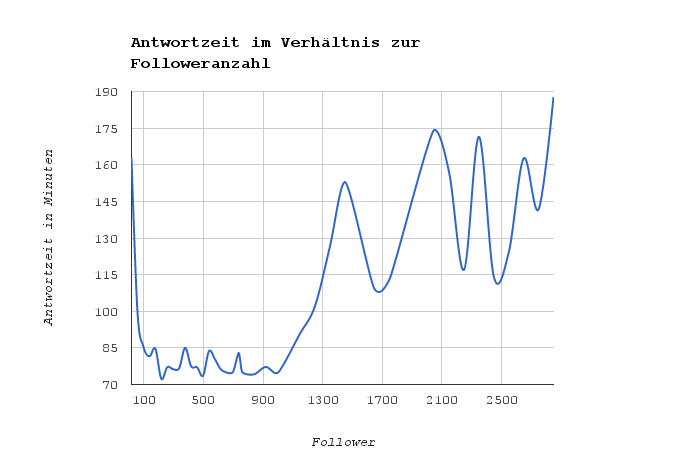
\includegraphics[scale=0.6]{diagramme/antwortzeitFollowerzahl.png}
\begin{center}
	\begin{tikzpicture}
		\begin{axis}[
		          width=\linewidth, % Scale the plot to \linewidth
		          legend pos = north west,
		          xlabel = {},
		          ylabel = {},
		          title={Länge von normalen Tweets und Fragen}
		        ]
			\addplot [mark=none,red]table [red,x index=0, y index=2, col sep=comma,mark=square] {csv/antwortzeitFollower.csv};
			\addlegendentry{Fragen}
		\end{axis}
\end{tikzpicture}
\end{center}
%%%%%%%%%%%%%%%%%

\subsubsection{Breite des Dialogbaums in Abhängigkeit von der  Followerzahl}

Einen weiteren Hinweis darauf, ob es sich um einen \textit{real dialog} handelt versprachen wir uns vom Blick auf die Breite des Dialogbaums. Unsere Überlegung war, dass der dialogische Charakter einer Twitter-Konversation durch einen \glqq schlanken\grqq\  Baum eher abgebildet wird, als durch einen \glqq breiten\grqq , da Breite nur darauf hindeutet, dass eine Frage von vielen Followern gelesen wurde und entsprechend singulär beantwortet wird, d.h., ohne nochmals auf andere Antworten einzugehen. Der Blick auf die Daten bestätigte unsere Vermutung: Zunächst kann man ablesen, dass eine übergroße Zahl von Dialogen genau aus 2 Tweets bestehen - einem initialem Tweet und einer Antwort. Ebenso jedoch kann abgelesen werden, dass mit zunehmender Followerzahl eines Users die Dialogbäume breiter werden. Betont werden muss, dass hier nicht betrachtet wird, wie viele unterschiedliche Teilnehmer sich an einem Dialog beteiligen, sondern wie viele Follower der Dialog-Eröffner hat. Es bleibt jedoch bei der Feststellung, dass eine größere Followerzahl mit einer größeren Breite eines Dialogbaums einhergeht und somit ein Dialog gewissermaßen mäandert.

\begin{table}[h]
\centering
\begin{tabular}{ccr}
Breite des Dialogbaums & Durchschnittliche Follower & Anzahl  \\
1                      & 1.506                       & 307.745 \\
2                      & 2.524                       & 33.297  \\
3                      & 3.979                       & 4.323   \\
4                      & 5.270                       & 890     \\
5                      & 8.022                       & 263     \\
6                      & 10.583                      & 83      \\
7                      & 20.603                      & 40     
\end{tabular}
\caption{My caption}
\label{my-label}
\end{table}

%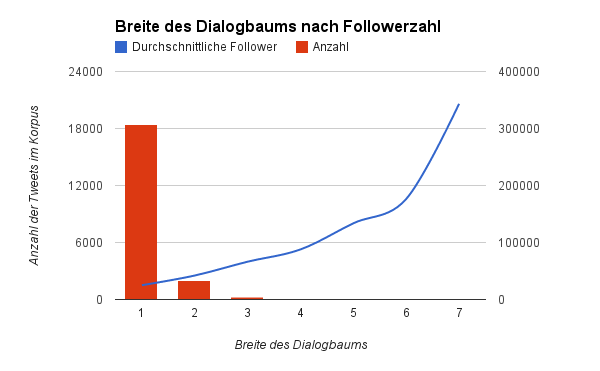
\includegraphics[scale=0.6]{diagramme/breiteFollower.png}
\begin{center}
	\begin{tikzpicture}
		\begin{axis}[
		          width=\linewidth, % Scale the plot to \linewidth
		          legend pos = north east,
		          xlabel = {},
		          ylabel = {},
		          title={Länge von normalen Tweets und Fragen}
		        ]
			\addplot [nodes near coords,mark=*,red] table [red,x index=0, y index=1, col sep=comma,mark=square] {csv/followerBreite.csv};
			\addlegendentry{Follower}
			\addplot [blue,mark=square] table [red,x index=0, y index=2, col sep=comma,mark=square] {csv/followerBreite.csv};
			\addlegendentry{Anzahl}
		\end{axis}

\end{tikzpicture}
\end{center}
\subsection{Dialoglänge und Dialogdauer}

Twitter ist ein extrem schnelllebiges Medium. Beiträge anderer User können sehr schnell aus dem Blickfeld der Follower geraten. Damit läuft eine erwünschte Konversationseröffung eines Users Gefahr, nicht wahrgenommen zu werden. Diese missglückten Versuche konnten von uns natürlich nicht nachgewiesen werden. Trotzdem konnten wir die Dauer von Konversation messen, indem wir die Differenz zwischen Dialogeröffnung und dem letzten Tweet des Dialoges zum Zeitpunkt der Erstellung des Korpus maßen. Die Dialoglänge selbst ermittelten wir, indem wir die Länge des längsten Pfades des Dialogbaums ermittelten.
Man kann erkennen, dass die übergroße Zahl von Dialogen eine Lebensdauer von weniger als 3 Stunden hat und zudem kaum Dialoge stattfinden, die länger als einen Tag dauern.
\begin{center}
	\begin{tikzpicture}
		\begin{axis}[ybar, nodes near coords,
		          width=\linewidth, % Scale the plot to \linewidth
			  axis y line*=left,
		          legend pos = north west,
		          xlabel = {Dialoglänge},
		          ylabel = {Anzahl der Dialoge},
		          title={Länge von normalen Tweets und Fragen}
		        ]
			\addplot [mark=none,red]table [x index=0, y index=3, col sep=comma] {csv/zeitspanneDialoglaenge.csv};
			\addlegendentry{Anzahl}
		\end{axis}
		\begin{axis}[
			hide x axis,
			axis y line*=right,
		          width=\linewidth, % Scale the plot to \linewidth
		          legend pos = north east,
			ylabel near ticks,
		          ylabel = Zeitdifferenz,
		        ]
			\addplot [mark=none,blue]table [x index=0, y index=2, col sep=comma] {csv/zeitspanneDialoglaenge.csv};
			\addlegendentry{Zeitdifferenz}
		\end{axis}
\end{tikzpicture}
\end{center}

\begin{table}[h]
\centering
\begin{tabular}{ccc}
Dialoglänge & Zeitdifferenz in Min & Anzahl Dialoge \\
2           & 120                  & 170.298        \\
3           & 164                  & 83.479         \\
4           & 199                  & 39.734         \\
5           & 223                  & 22.168         \\
6           & 256                  & 11.640         \\
7           & 305                  & 7.109          \\
8           & 308                  & 4.074          \\
9           & 345                  & 2.799          \\
10          & 405                  & 1.671          \\
11          & 392                  & 1.089          \\
12          & 447                  & 674            \\
13          & 410                  & 522            \\
14          & 593                  & 373            \\
15          & 552                  & 236           
\end{tabular}
\caption{My caption}
\label{my-label}
\end{table}



\subsection{Dialog und Fragen}

Besonders interessiert hat uns, ob Twitter genutzt wird, um Fragen zu stellen und zu hoffen, diese beantwortet zu bekommen. 

Eine zentrale Aufgabe stellte dabei die Identifizierung von Fragen dar. Wir gingen davon aus, dass aufgrund der Beschränkung auf 140 Zeichen viele Twitter-Nutzer auf die Angabe von Fragezeichen verzichten würden:

\textit{Wieso flüstern die so maaaan} (ID: 318495612649762816)


Daher untersuchten wir einen Tweet zusätzlich darauf, ob er sogenannte w-Wörter (\textit{wer, wie, was, wodurch ...}) enthielt (satzinitial sowie satzintern) und ermittelten folgende Verteilung hinsichtlich der Attribute Fragezeichen und w-Wörter:

\begin{table}[h]
\centering
\begin{tabular}{lr}
Fragezeichen                                & 2.374.174 \\
Tweet mit w-Wort                            & 588.322   \\
Tweet mit initialem w-Wort mit Fragezeichen & 92.077    \\
Tweet mit initalem w-Wort ohne Fragezeichen & 51.465   
\end{tabular}
\caption{My caption}
\label{my-label}
\end{table}

Aus dieser Verteilung kann abgelesen werden, dass der potentielle Zugewinn durch das Betrachten von Tweets mit initalen w-Wörtern und ohne Fragezeichen gering wäre, zumal eine eindeutige Klassifizierung als Frage dann immer noch nicht gegeben wäre:


\textit{Wen du endlich ewachsen bist und mich in Ruhe lässt lass es mich wissen ansonsten viel spaß noch! Wirst schon sehen!} (ID: 318501739030536192)

Da es bei einer so großen Datenmenge aus Geschwindigkeitsgründen nicht möglich ist, Fragen akkurat und linguistisch korrekt anhand syntaktischer Merkmale zu identifizieren, mussten wir uns einer Näherungslösung bedienen. Jeweils 100 zufällig gewählte Tweets, die entweder als wh-question, als Tweet mit Fragezeichen oder als Nicht-Frage getagged waren, überprüften wir händisch und ermittelten folgende Ergebnisse:

\begin{table}[h]
\centering
\begin{tabular}{lccc}
        & wh\_question=1 & question\_mark=1 & is\_question=0 \\
richtig & 73           & 100            & 100            \\
falsch  & 27           & 0              & 0             
\end{tabular}
\caption{My caption}
\label{my-label}
\end{table}

Wir mussten erkennen, dass nicht nur der Anteil potentieller Fragen, bei denen auf ein Fragezeichen verzichtet wurde, gering war, sondern gleichzeitig auch die Überprüfung hinsichtlich der Existenz von w-Wörtern eine Fehlerquote von 27 \% aufwies. Gleichzeitig war in unserer Stichprobe jeder der untersuchten Tweets mit Fragezeichen tatsächlich eine Frage. Das Ergebnis dieses Test widersprach unserer Erwartung, dass auf den Einsatz von Fragezeichen verzichtet würde. Das Attribut \texttt{question\_mark} stellte sich als zuverlässigstes Indiz zur Fragenerkennung heraus. Wir beschränkten uns daher auf dieses Attribut, um Tweets als Fragen zu identifizieren.

\subsubsection{Länge von normalen Tweets und Fragen}

Zunächst warfen wir einen Blick auf die durchschnittliche Tweetlänge. Unsere Vermutung war, dass es bei den Fragen einen höheren Anteil von Nachrichten mit geringer Länge geben würde, da oftmals einfache w-Wörter gesendet werden. Dieser Eindruck bestätigte sich jedoch nicht. Stattdessen folgen Fragen ebenso wie normale Tweets dem selben Muster, dass die maximal mögliche Zeichenanzahl ausgenutzt wird. Interessant ist die Tatsache, dass sowohl in Fragen als auch normalen Tweets ein Maximum an Tweets bei der Länge 136 gemessen wurde. Dies deutet darauf hin, dass User, die an die maximal zulässige Marke von 140 Zeichen kommen, ihren Tweet kürzen, indem lange Wörter durch kürzere ersetzt werden.

\begin{center}
	\begin{tikzpicture}
		\begin{axis}[
			axis y line*=left,
		          legend pos = south west,
		          width=\linewidth, % Scale the plot to \linewidth
		          xlabel = {Anzahl Zeichen},
			ylabel = Anzahl Tweets,
		          title={Länge von normalen Tweets und Fragen}
		        ]
			\addplot [mark=none,red]table [x index=0, y index=1, col sep=comma,mark=square] {csv/laenge.csv};
			\addlegendentry{Fragen}
		\end{axis}

		\begin{axis}[
			hide x axis,
			axis y line*= right,
		          legend pos = south east,
		          width=\linewidth, % Scale the plot to \linewidth
			ylabel near ticks,
		          ylabel = Anzahl Fragen,
		        ]
			\addplot [mark=none,blue] table [x index=0, y index=2, col sep=comma] {csv/laenge.csv};
			\addlegendentry{Tweets}
		\end{axis}
\end{tikzpicture}
\end{center}

\subsubsection{Frage-Antwort-Ratio}

Wir wollten wissen, wie die Länge einer Frage die Chance erhöht, auch eine Antwort zu erhalten und nicht in der Tweetflut der Follower unterzugehen. Wir vermuteten, dass eine längere und damit klarer formulierte Frage mehr Antworten bzw. überhaupt eine Antwort erhalten sollte, als kürzere. Um diese Frage beantworten zu können, ermittelten wir eine \textit{Frage-Anwort-Ratio} sämtlicher Fragen-initialer Dialoge mit jeweils der gleichen Länge der Frage. Dabei ermittelten wir somit für beantwortete Fragen schlicht die Zahl der Antworten. Eine Frage mit 3 Antworten hat somit eine $Frage-Antwort-Ratio = 3$. Da viele Fragen keine Antwort erhalten wird sich die $Frage-Antwort-Ratio$ für jeweilige Zeichenlängen maximal $1$ erreichen.

\begin{center}
	\begin{tikzpicture}
		\begin{axis}[
			axis y line*=left,
		          legend pos = south west,
		          width=\linewidth, % Scale the plot to \linewidth
		          xlabel = {Anzahl Zeichen},
			ylabel = Frage-Antwort-Ratio,
		          title={Frage-Antwort-Ratio aller Fragen}
		        ]
			\addplot [mark=none,red]table [x index=0, y index=1, col sep=comma,mark=square] {csv/faRatioUnbeantwortet.csv};
			\addlegendentry{Frage-Antwort-Ratio}
		\end{axis}

		\begin{axis}[
			hide x axis,
			axis y line*= right,
		          legend pos = south east,
		          width=\linewidth, % Scale the plot to \linewidth
			ylabel near ticks,
		          ylabel = Anzahl Tweets,
		        ]
			\addplot [mark=none,blue] table [x index=0, y index=2, col sep=comma] {csv/faRatioUnbeantwortet.csv};
			\addlegendentry{Anzahl Tweets}
		\end{axis}
\end{tikzpicture}
\end{center}

Man kann erkennen, dass die Frage-Antwort-Ratio bei sehr kurzen Fragen ohnehin sehr gering ist. Ab einer Zeichenlänge von 40 steigt sie spürbar an, lässt danach jedoch keine weitere Tendenz zum Anstieg erkennen. Dies spiegelt die erwähnte Gefahr wieder, dass eine Frage unbeantwortet bleibt.

In einem zweiten Schritt untersuchten wir die Frage-Antwort-Ratio bei allen den Fragen, die mindestens eine Antwort erhielten. Aus diesen Gründen ist die $Frage-Antwort-Ratio >= 1$. Auffällig ist die kontinuierlich ansteigende Kurve der Frage-Antwort-Ratio mit zunehmender Länge der initialen Frage.  

\begin{center}
	\begin{tikzpicture}
		\begin{axis}[
			axis y line*=left,
		          legend pos = south west,
		          width=\linewidth, % Scale the plot to \linewidth
		          xlabel = {Anzahl Zeichen},
			ylabel = Frage-Antwort-Ratio,
		          title={Frage-Antwort-Ratio aller Fragen mit mindestens einer Antwort}
		        ]
			\addplot [mark=none,red]table [x index=0, y index=1, col sep=comma,mark=square] {csv/faRatioBeantwortet.csv};
			\addlegendentry{Frage-Antwort-Ratio}
		\end{axis}

		\begin{axis}[
			hide x axis,
			axis y line*= right,
		          legend pos = south east,
		          width=\linewidth, % Scale the plot to \linewidth
			ylabel near ticks,
		          ylabel = Anzahl Tweets,
		        ]
			\addplot [mark=none,blue] table [x index=0, y index=2, col sep=comma] {csv/faRatioBeantwortet.csv};
			\addlegendentry{Anzahl Tweets}
		\end{axis}
\end{tikzpicture}
\end{center}

\subsubsection{Fragen und Antworten im Tagesverlauf}
Wir wollten wissen, ob man aus den erhobenen Daten Hinweise gewinnen kann, zu welcher Tageszeit das Stellen einer Frage auf Twitter besonders sinnvoll erscheint, wenn ein User tatsächlich an einer Antwort interessiert ist. 

Zunächst interessierte uns, wie schnell ein User zu welcher Tageszeit im Durchschnitt eine Antwort auf seine Frage erhielt. Wir vermuteten, dass eine Nachts gesendete Frage viel länger auf eine Beantwortung warten müsse, als eine zur Prime-Time veröffentlichte Frage. Die Daten offenbarten folgende Muster:

\pgfplotstableread[col sep=comma]{csv/sheet20.csv}\datatable
\makeatletter
\pgfplotsset{compat=1.6,
    /pgfplots/flexible xticklabels from table/.code n args={3}{%
        \pgfplotstableread[#3]{#1}\coordinate@table
        \pgfplotstablegetcolumn{#2}\of{\coordinate@table}\to\pgfplots@xticklabels
        \let\pgfplots@xticklabel=\pgfplots@user@ticklabel@list@x
    }
}
\makeatother


\begin{center}
    \begin{tikzpicture}
        \begin{axis}[
           % ycomb,
            width=\linewidth, % Scale the plot to \linewidth
            %legend pos = north west,
           % visualization depends on={value \thisrow{Stunde} \as \labela}, % note the value prefix
            xlabel=Wochentag-Stunde,
            ylabel=Antwortzeit,
          flexible xticklabels from table={csv/sheet20.csv}{Stunde}{col sep=comma},
          xticklabel style={rotate=90}, % To make sure the text labels are nicely aligned
         xtick=data,
            title={Wartezeit zur ersten Antwort nach Wochentag-Stunde}
            ]
           \addplot [red,mark=none] table [x expr=\coordindex, y index=2, col sep=comma] {csv/sheet20.csv};
            %\addlegendentry{}
        \end{axis}
\end{tikzpicture}
\end{center}

Die durchschnittlich kürzeste Antwortzeit mit 64 Minuten entdeckten wir Dienstags um 21 Uhr. Es könnte also vermutet werden, dass die Abendstunden ein guter Zeitraum sind, um Fragen zu stellen und schnell beantwortet zu bekommen. Wenig verwunderlich finden sich die Maximalwerte bei den Antwortzeiten in den Nachtstunden. So können die 3 auffälligen Werte sämtlich in den sehr frühen Morgenstunden gefunden werden (Maximalwert 294 Minuten am Samstagmorgen 4 Uhr).

Neben der Geschwindigkeit, mit der eine Frage eine Antwort erhält gibt es natürlich noch eine zweite Kategorie, die für einen Fragensteller interessant ist: die Menge der Antworten auf eine Frage. Um diesen Aspekt zu beurteilen betrachteten wir die unterschiedlichen Wochentage über einen Zeitraum von einem Monat. Wir unterteilten jeden einzelnen Tag nochmals in seine 24 Stunden und ermittelten die Frage-Antwort-Ratio für diese Zeiträume.

\pgfplotstableread[col sep=comma]{csv/frageAntwortWochentag.csv}\datatable
\makeatletter
\pgfplotsset{compat=1.6,
    /pgfplots/flexible xticklabels from table/.code n args={3}{%
        \pgfplotstableread[#3]{#1}\coordinate@table
        \pgfplotstablegetcolumn{#2}\of{\coordinate@table}\to\pgfplots@xticklabels
        \let\pgfplots@xticklabel=\pgfplots@user@ticklabel@list@x
    }
}
\makeatother


\begin{center}
    \begin{tikzpicture}
        \begin{axis}[
        %    ycomb,
            width=\linewidth, % Scale the plot to \linewidth
            %legend pos = north west,
           % visualization depends on={value \thisrow{Stunde} \as \labela}, % note the value prefix
            xlabel=Wochentag-Stunde,
            ylabel=Frage-Antwort-Ratio,
          flexible xticklabels from table={csv/frageAntwortWochentag.csv}{F}{col sep=comma},
          xticklabel style={rotate=45}, % To make sure the text labels are nicely aligned
         xtick=data,
            title={Frage-Antwort-Ratio nach Wochentag-Stunde}
            ]
           \addplot [red,mark=none] table [x expr=\coordindex, y index=3, col sep=comma] {csv/frageAntwortWochentag.csv};
            %\addlegendentry{}
        \end{axis}
\end{tikzpicture}
\end{center}

Auch in diesem Fall sind die Einbrüche in den Nachtstunden auf den ersten Blick erkennbar. Ebenso erkennbar sind jedoch die immer wiederkehrenden Muster in den Abendstunden. Während in den Abendstunden nach 21 Uhr die Frage-Antwort-Ratio stets absinkt, erreicht sie gegen Mitternacht jeweils ihr Hoch. Dies gilt für sämtliche Wochentage. Man scheint also die Medienkonsum-Gewohnheiten der User entdecken zu können: Während der Abend gesellschaftliche Aktivitäten gehören scheint für User der Blick auf den Twitter-Account vor dem Zu-Bett-Gehen üblich zu sein. Die höchste Fragen-Antwort-Ratio wird Samstag Mitternacht erzielt.





\end{document}



